\RequirePackage{ifpdf}
\documentclass[a4paper,11pt]{kth-mag}

\usepackage[T1]{fontenc}
\usepackage{textcomp}
\usepackage{lmodern}
\usepackage[latin1]{inputenc}
\usepackage[swedish,english]{babel}
\usepackage{modifications}

%Egna paket
%For swedish
\usepackage[swedish]{babel}

%For comments
\usepackage{verbatim}

%For graphics
\usepackage{graphicx}
\usepackage[section]{placeins}%Makes floats stay in place
\usepackage{caption}
\usepackage{subcaption}
\captionsetup{compatibility=false} %Problem with subcaption workaround

\usepackage{gensymb} % Provides \degree \textdegree


%Egna kommandon
%\let\oldsection\section
%\renewcommand{\section}[1]{
%\FloatBarrier
%\oldsection{#1}
%\FloatBarrier
%}




\title{Efficient features for representing hand shape in images}

\subtitle{Using a classeme-based approach}

\foreigntitle{Effektiva visuella formdeskriptorer för handigenkänning}
\author{Patrik Berggren}
\date{Juni 2014}
\blurb{Master's Thesis at NADA\\Supervisor: Hedvig Kjellström\\Examiner: Danica Kragic}
\trita{TRITA xxx yyyy-nn}
\begin{document}
\frontmatter
\pagestyle{empty}
\removepagenumbers
\maketitle
\selectlanguage{english}


%Acknowledgements
%Hedvig såklart för handledning, ideer, kritik, kommentarer
%Akshaya hjälp med att sätta upp systemet, hans master uppsats, references, handledning?
% Hjälp vid presentationsförberedelser, hjälp med korrekturläsning

\begin{abstract}
%TODO
Abstract to come
\end{abstract}
\clearpage
\begin{foreignabstract}{swedish}
%TODO
Abstract to come
\end{foreignabstract}
\clearpage
\tableofcontents*
\mainmatter
\pagestyle{newchap}

\section{Introduction}
Today, there is a shift in the ways we interact with computers taking place.
Previously, it has mainly been through keyboards and mouse, but today you find that there are touchscreens, wii, kinect and speech-recognition.
The trend is that interactions become more intuitive and making gestures with ones hands can certainly be very intuitive.
Therefore, a lot of research have been done to investigate what methods can be used for hand pose estimation (HPE).
%TODO applikationer

However, hand pose estimation is difficult and since no generally applicable method for it exists, many different approaches have been tested.
One of the biggest challenges is that the hand can move in many different ways i.e. have many degrees of freedom.
Furthermore the hand can move very rapidly and is also able to occlude itself in many poses.
Both the high dimensionality and self occlusion contributes to the discontinuity and ambiguity that exists between the image and the hand pose space.
The goal of this thesis is, nevertheless, to find ways to overcome these problems to some degree and to hopefully contribute with a new HPE method using a new image descriptor.

The basis of this thesis is an earlier master thesis done by Akshaya Sridatta Thippur \cite{akshayaMaster} in which he investigated which image features was most suitable for HPE.
This thesis will expand that idea and continue from one of the image features that was judged to have overall good properties, namely Histograms of Oriented Gradients (HOG features).
 
\chapter{Theory and Background}
This section follows a top-down approach where the overall process of hand estimation methods is presented in section~\ref{sec:overview} followed by a more detailed discussion about the different aspects of hand pose estimation.

\section{Overview}
\label{sec:overview}
In this section a table of related work is presented to give the reader an overview.
Details of the different aspects are then discussed in later sections.
The main objective of hand estimation is of course to take an image containing a hand and returning the corresponding hand pose.
However, there is several steps that happens in between more or less regardless of method used.
First of all, the hand must be detected in the image and this is in fact a separate problem from hand pose estimation, although hand pose estimation of course depends a lot on the former (see \cite{survey} for a survey of different detection papers).
It is also the case that in many detection methods similar image features are used as in estimation, in \cite{realTime} HOG features are used for instance which we will see is a common choice for hand pose estimation as well.
After the hand is detected, it is common to assume that the hand is segmented out i.e. that the background is removed, although not all methods relies on this\cite{clutter}.

It is from this point that we start to extract information concerning the pose of the hand.
One might at first imagine that the image pixels are feed into a machine learning algorithm directly, but that gives poor results.
Individual pixels tells very little about the pose and so to obtain any meaningful information, complex relations would have to be found which puts a lot of burden on the machine learning algorithm.
Instead, most methods use a step in between which extracts what is called image features, which basically is a set of values that are meant to capture some feature of the image that is more relevant for pose estimation than individual pixels.
Most of those features builds on the assumption that what we are interested in is edges since the form of the hand is generally enough to determine what pose it is in. 
There are, however, a range of different features and those will be discussed more in section~\ref{sec:feature}.

Except from different image feature, there is a different aspect of hand pose estimation that also divides pose estimation methods, which is discriminative versus generative approaches.
When using a discriminative approach the mapping between features and pose space is found directly.
That is, the mapping is determined by some type of regression method that estimates the mapping based on a set of training data consisting of pairs of feature values and corresponding poses.
However, in a generative approach there is no explicit mapping that is computed, but the problem is rather reduced to an optimization problem.
This is done by using a model of the hand so that a pose can be used as input to generate a hand image from which image features are extracted.
The idea is to generate such hand images from different hand poses until we get image features that are close to the observed features.
Discriminative versus generative approaches are discussed in more detail in section~\ref{sec:discgen}.

There are still further aspects of hand pose estimation that deserves a discussion since they can have a big impact on the accuracy of the methods.
One of those is the possibility to instead of having a single camera, the scene is captured as a multi-frame from different view angles.
Another aspect that is sometimes used is to rely on temporal constraints on the pose, which means that it is assumed that poses doesn't change too fast so that we can use the estimated pose from a previous frame to determine which poses are likely now.
Both of these methods can remove some of the ambiguity in the mapping between features and pose space and the multi-view approach can to a large degree remove self-occlusion problems.

All the above mentioned aspects of hand pose estimation can in fact be applied to estimate other things, and most commonly, hand pose estimation is compared to human pose estimation which shows many similarities. 
One might also consider situations in which hands interact with objects which can be a considered a more realistic scenario seen as the hand often interacts with objects. 

Table~\ref{tab:overview} shows some works concerning mainly hand and human pose estimation.
The collection is by no means meant to be representative of the research in those areas, but is rather meant to give the reader an overview of the papers concerning estimation methods cited in this thesis.
The columns of the table shows the different aspects mentioned above which is also discussed later in this chapter.
The first, Type, is to tell what is estimated, meaning if the paper is concerned with human or hand pose estimation.
The third column, Pose space, determines what kind of model is used for the body/hand.
Discrete in this context normally means that the paper is concerned with classes of gestures/poses of some kind, whilst continuous or an exact number of degrees of freedom (DOF) means that the estimation is done for a model with that many degrees of freedom.
Disc/Gen stands for discriminative and generative.
The view columns describes what kind of setting the method is tested in i.e. single viewpoint or multiple viewpoints.
Finally, the Temporal column describes if the method used takes into account temporal constraints.

\begin{table}[!ht]
    %\advance\leftskip-4cm
    \noindent\makebox[\textwidth]{%
    \begin{tabular}{|c|c|c|c|c|c|c|}
        \hline
        First author & Type & Pose space & Feature & Disc/Gen & View & Temporal
        \\
        \hline
        Jing \cite{temporal} 
                                    & Hand
                                    & Discrete 
                                    & HOG
                                    & Disc 
                                    & Single
                                    & Yes
        \\
        \hline
        Mihalache \cite{RGB}     
                                    & Hand
                                    & Discrete 
                                    & HOG+fingertips 
                                    & Disc 
                                    & RGB-D 
                                    & No
        \\
        \hline
        Murase \cite{keyboard}     
                                    & Hand
                                    & Discrete %keys
                                    & HOG 
                                    & Disc %adaboost 
                                    & Single 
                                    & No
        \\
        \hline
        Thangali \cite{signs}
                                    & Hand
                                    & Discrete
                                    & HOG
                                    & Disc% (SVM)
                                    & Single
                                    & Yes
        \\
        \hline
        Romero \cite{cyberglove} 
                                    & Hand
                                    & Discrete 
                                    & Cyberglove 
                                    & Gen
                                    & Cyberglove
                                    & Yes
        \\
        \hline
        Campos \cite{regressionBased}     
                                    & Hand
                                    & 26 DOF 
                                    & Shape context 
                                    & Disc%, RVM 
                                    & Single+multi 
                                    & No
        \\
        \hline
        Athitsos \cite{clutter} 
                                    & Hand
                                    & 20 DOF
                                    & DCD to representatives 
                                    & Disc
                                    & Single
                                    & No
        \\
        \hline
        Oikonomidis \cite{fullDOF}
                                    & Hand+Object
                                    & 26 DOF 
                                    & SIFT
                                    & Gen% (PSO)
                                    & Multi 
                                    & No
        \\
        \hline
        Romero \cite{monocular}     
                                    & Hand+Object
                                    & 31 DOFs 
                                    & HOG %pyramidHOG 
                                    & Disc% k-NN %LSH
                                    & Single
                                    & Yes
        \\
        \hline
        Romero \cite{nonparametric} 
                                    & Hand+Object
                                    & Continous %Står inte DOF
                                    & HOG
                                    & Disc 
                                    & Single
                                    & Yes
        \\
        \hline
        Kaaniche \cite{tracking}
                                    & Human
                                    & Discrete
                                    & HOG
                                    & Disc% (SVM)
                                    & Single
                                    & Yes
        \\
        \hline
        Dalal \cite{HOG}    & Human 
                            & Discrete
                            & HOG
                            & Detection
                            & Single
                            & No
        \\
        \hline
        Lin \cite{humanBody} 
                                    & Human
                                    & 28 DOFs 
                                    & HOG
                                    & Disc 
                                    & Single 
                                    & No
        \\
        \hline
        Shakhnarovich \cite{PSH} 
                                    & Human
                                    & 13 DOFs 
                                    & Edge direction histogram %Multi-scaled edge diretion histogram 
                                    & Disc
                                    & Single
                                    & No
        \\
        \hline
        Lin \cite{humanBody} 
                                    & Human
                                    & 28 DOFs 
                                    & HOG
                                    & Disc 
                                    & Single
                                    & No
        \\
        \hline
        Johnson \cite{combining}     
                                    & Human
                                    & 30 DOFs
                                    & HOG+seg cues 
                                    & Disc 
                                    & SIngle
                                    & No
        \\
        \hline
        Poppe \cite{exampleBased}     
                                    & Human
                                    & 34 DOFs %From other paper about humanEva
                                    & HOG %nonOverlapp
                                    & Disc %k-NN %Exact?
                                    & Single+multi
                                    & No
        \\
        \hline
        Onishi \cite{3Dhuman}     
                                    & Human
                                    & 24 DOFs 
                                    & HOG %Overlapp, unsigned 
                                    & Disc%, linear SVM
                                    & Single 
                                    & No
        \\
        \hline
        Andriluka \cite{pictorial}     
                                    & Human
                                    & 40 DOFs 
                                    & Shape context 
                                    & Gen
                                    & Single+multi 
                                    & No
        \\
        \hline
        Agarwal \cite{recovering3D}     
                                    & Human
                                    & 55 DOFs 
                                    & Shape context 
                                    & Disc%, RVM/SVM 
                                    & Single 
                                    & Yes
        \\
        \hline
        Lowe \cite{SIFT}            & Object 
                                    & Discrete 
                                    & SIFT
                                    & Disc% k-NN
                                    & Single
                                    & No
        \\
        \hline
        Belongie \cite{shape}     
                                    & Miscellaneous 
                                    & Discrete %From other paper about humanEva
                                    & Shape context %nonOverlapp
                                    & Disc %k-NN %Exact?
                                    & Single
                                    & No
        \\
        \hline
    \end{tabular}}
    \caption{
The papers are denoted by the first authors surname and the paper is also referenced.
The Type column is to tell what is estimated, meaning if the paper is concerned with human or hand pose estimation.
The third column, Pose space, determines what kind of model is used for the body/hand.
Discrete in this context normally means that the paper is concerned with classes of gestures/poses of some kind, whilst continuous or an exact number of degrees of freedom (DOF) means that the estimation is done for a model with that many degrees of freedom.
Disc/Gen stands for discriminative and generative.
The view columns describes what kind of setting the method is tested in i.e. single viewpoint or multiple viewpoints.
Finally, the Temporal column describes if the method used takes into account temporal constraints.
}
    \label{tab:overview}
\end{table}

\section{Human vs Hand estimation}
As table~\ref{tab:overview} shows some of the related work are human pose estimation and not hand pose estimation.
The reason for this is that human pose estimation have much in common with hand pose estimation.
For one thing, a human pose is often modeled with similar dimensions as the hand is modeled, but more importantly the arms, legs, and head of the body plays a similar role as the fingers of the hand.
However, there are some differences and the two problems faces slightly different problems.
For human pose estimation the segmentation will be more difficult because our method must be robust against a wide range of clothing, whilst hand estimation can generally suppose that the hand is not occluded with the exception of a ring or similar.
However, when dealing with human poses it is often assumed that it is a standing pose as one of the main applications is pedestrian detection and pose estimation.
For hands it is difficult to make such assumptions.
Furthermore, hand pose estimation suffers from difficulty in distinguishing between fingers, and also has a great degree of self occlusion in many poses. 
Also, related to this is the fact that, as in \cite{combining}, human pose estimation can be approached by first detecting the individual limbs and then estimating the pose whilst this is very difficult to do for hand pose estimation since fingers aren't easily distinguishable.

Another type of scenario that is of interest is when a hand interacts with an object.
In situations like hand signs and gestures, approaches with no object is of course useful, but it is arguably more realistic with a scenario where a hand interacts with an object.
Applications that directly requires this is for instance when a robot needs to learn a task by demonstration which can include grasping objects in different ways as in \cite{fullDOF}.


\section{Pose space}
When discussing pose or joint space there is mainly two aspects that is of interest.
Firstly, we are interested in which poses are possible and in that sense makes up the pose space, and secondly we are interested in how poses are represented.
We begin our discussion with a short description of the hand anatomy since that must necessarily be our starting point in forming a hand model.

\subsection{Hand anatomy}
It is quite apparent that the hands anatomy will be the basis for any hand model, but more importantly it can tell us specifically which aspects are important to capture and which we might discard in order to get a simpler model.
On one hand a too simple hand model will result in an unnatural model where a lot of possible hand motions are impossible in the model.
However, one doesn't want a too complex model either since that will make hand pose estimation harder.

Figure~\ref{fig:hand} shows a X-ray of a human hand which normally have 27 bones\cite{anatomy}. 
The bones at the base of the palm is called Carpals from which the base of the fingers stretch out.
Each finger consists of bone parts starting from the base, metacarpals, proximal phalanges, intermediate (or middle) phalanges, and distal phalanges, except for the thumb which doesn't have the intermediate phalanges.
As can be seen in the figure the joints are named according to which bones they connect.

\begin{figure}[!ht]
    \centering
    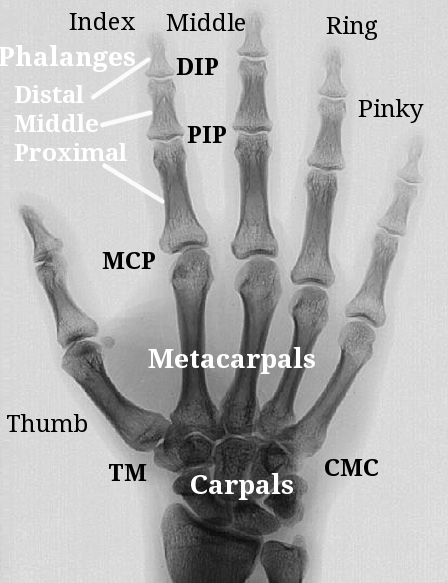
\includegraphics[width=0.5\textwidth]{images/handskeletone/labeledSkeletone.png}
    \caption{X-ray of a hand with labels for joint and bone names.}
    \label{fig:hand}
\end{figure}

One might be surprised at the many bones in the hand, but what is really  of interest to us is what degrees of freedom exists.
That is, in how many different ways can we move the hand.
It is here necessary to distinguish between two different kinds of freedom.
Firstly we have the DOF (degrees of freedom) that the hand can move in on itself.
However, we also have DOF which the hand physically can be put into, but is not capable of doing on its own.
For instance, each finger can be slightly rotated if a torque is put on it, but there is no muscle that can perform this motion.
Apart from that, we must also consider that many DOFs are restricted in their range.
There is for instance a limit to how far back one can pull the fingers.
As if all this is not enough we can as Akshaya points out include a lot of other things in our model such as skin-color, subject-specific joint constraints, and hand size \cite{akshayaMaster}.
The conclusion is that some simplifications must be done to obtain a workable hand model.

\subsection{Representation}
The pose space representation is normally represented by the joint angles which models the kinematics of the hand and neglecting aspects not affecting the pose.
As the previous section shows the actual anatomy of the hand is surprisingly complex, although the pose of the hand is exclusively determined by the phalanges and metacarpals which bones constitutes 19 out of the 27 bones of the hand.
Although, a model of the hand should probably include as much as 35 or more dimensions to be realistic\cite{akshayaPaper}, there are some simplifications that can be made so that a hand can be represented with considerable fewer degrees of freedom \cite{review}.
However, this depends on whatever dynamic constraints are modeled or not.
It is for instance commonly noticed that the angle between the DIP and PIP joints are related by the equation $\Theta_{DIP} \approx \frac{2}{3}\Theta_{PIP}$ where $\Theta$ represents the angle of the joint\cite{review}.
Using such dynamic constraints can however be oversimplifying since they can be broken if an external force is applied which can easily be the case if the hand interacts with other objects or even with itself (i.e. fingers pushing against other fingers).

As noted in \cite{review} most models use one degree of freedom (DOF) for the DIP and PIP joints, two DOF for the MCP joints, two DOF for the TM joint and 6 DOF for the wrist. 
This yields a total of 27 DOF excluding the additional dimensions that are normally included for the camera position and angle.
Although, \cite{clutter} models a pose without the wrist and thus reducing the dimensionality.
However modeling the palm as a rigid body is not realistic and has therefore been varied in some models for the MCP joints are extended with an additional degree (twisting) and where the CMC joints are also modeled as one DOF joints (flextion/extension) \cite{review}.

One problem in hand pose estimation is that regardless of which pose space is used it is difficult to obtain training data with ground truth values for the pose.
A common solution to this problem is to use programs such as libHand \cite{libhand} that generates a picture from a pose setting.
This is of course in an artificial context, but it has been observed that learning from such generated pictures doesn't prohibit estimation of real images \cite{regressionBased}.

Lastly, it should be noted that it is not always possible to use an explicit kinematic model of the hand.
As can be seen in table~\ref{tab:overview} there are several studies where the goal haven't been to estimate a kinematic model of the hand, but rather to classify different poses into discrete sets.
Applications include classifying grasping actions \cite{cyberglove}, gestures \cite{tracking}, sign language \cite{signs}, and virtual keyboards \cite{keyboard}.

\section{Image features}
\label{sec:feature}
When doing HPE and image recognition in general one normally doesn't work directly with the pixels of the image.
Instead, one extract what is called image features from the image that are meant to capture some feature that is less local than a single pixel.
Some of the features that are regularly used in HPE is Histogram of Oriented Gradients (HOG)\cite{HOG,monocular,3Dhuman}, silhouette-based features \cite{fullDOF}, Scale-invariant feature transform (SIFT) \cite{SIFT},  Hu-moments, shape context Descriptors \cite{shape,recovering3D,regressionBased} and others.  

This thesis focuses on HOG features, but other features certainly have merits as well.
For instance, SIFT features, which for instance is used in \cite{SIFT}, are invariant to scaling and rotation which is a good property of an image feature since neither scaling nor rotation is relevant to the actual pose. 
Although HOG features doesn't display these properties they are at least robust against small changes \cite{monocular}.

\subsection{HOG features}
HOG (histogram of oriented gradients) features was first presented by Dalal and Triggs 2005 and was in the initial paper used to estimate and detect human poses\cite{HOG}.
The idea is that images can be described by the intensity gradients that it contains.
That is, the directions in which the intensity increases the most in different parts of the image.
The first step in computing a HOG feature is dividing the image into cells, which is a rectangular grid over the image.
The gradients is then computed in each cell and the distribution is recorded in a histogram.
It is common to ignore orientation of the gradient so that opposite pointing gradients are put into the same bin, but here again it is possible to use bins from 0 to $360\degree$.
To make the features more robust from illumination and shadow differences the feature values are sometimes normalized over blocks of several cells where the intensity gradients have been normalized \cite{HOG}, although this isn't necessary (\cite{exampleBased} for instance doesn't do this).
As can be seen in figure~\ref{fig:HOG_girl} the histograms can be said to roughly keep information about the edges in the image. 
\begin{figure}[!ht]
    \centering
    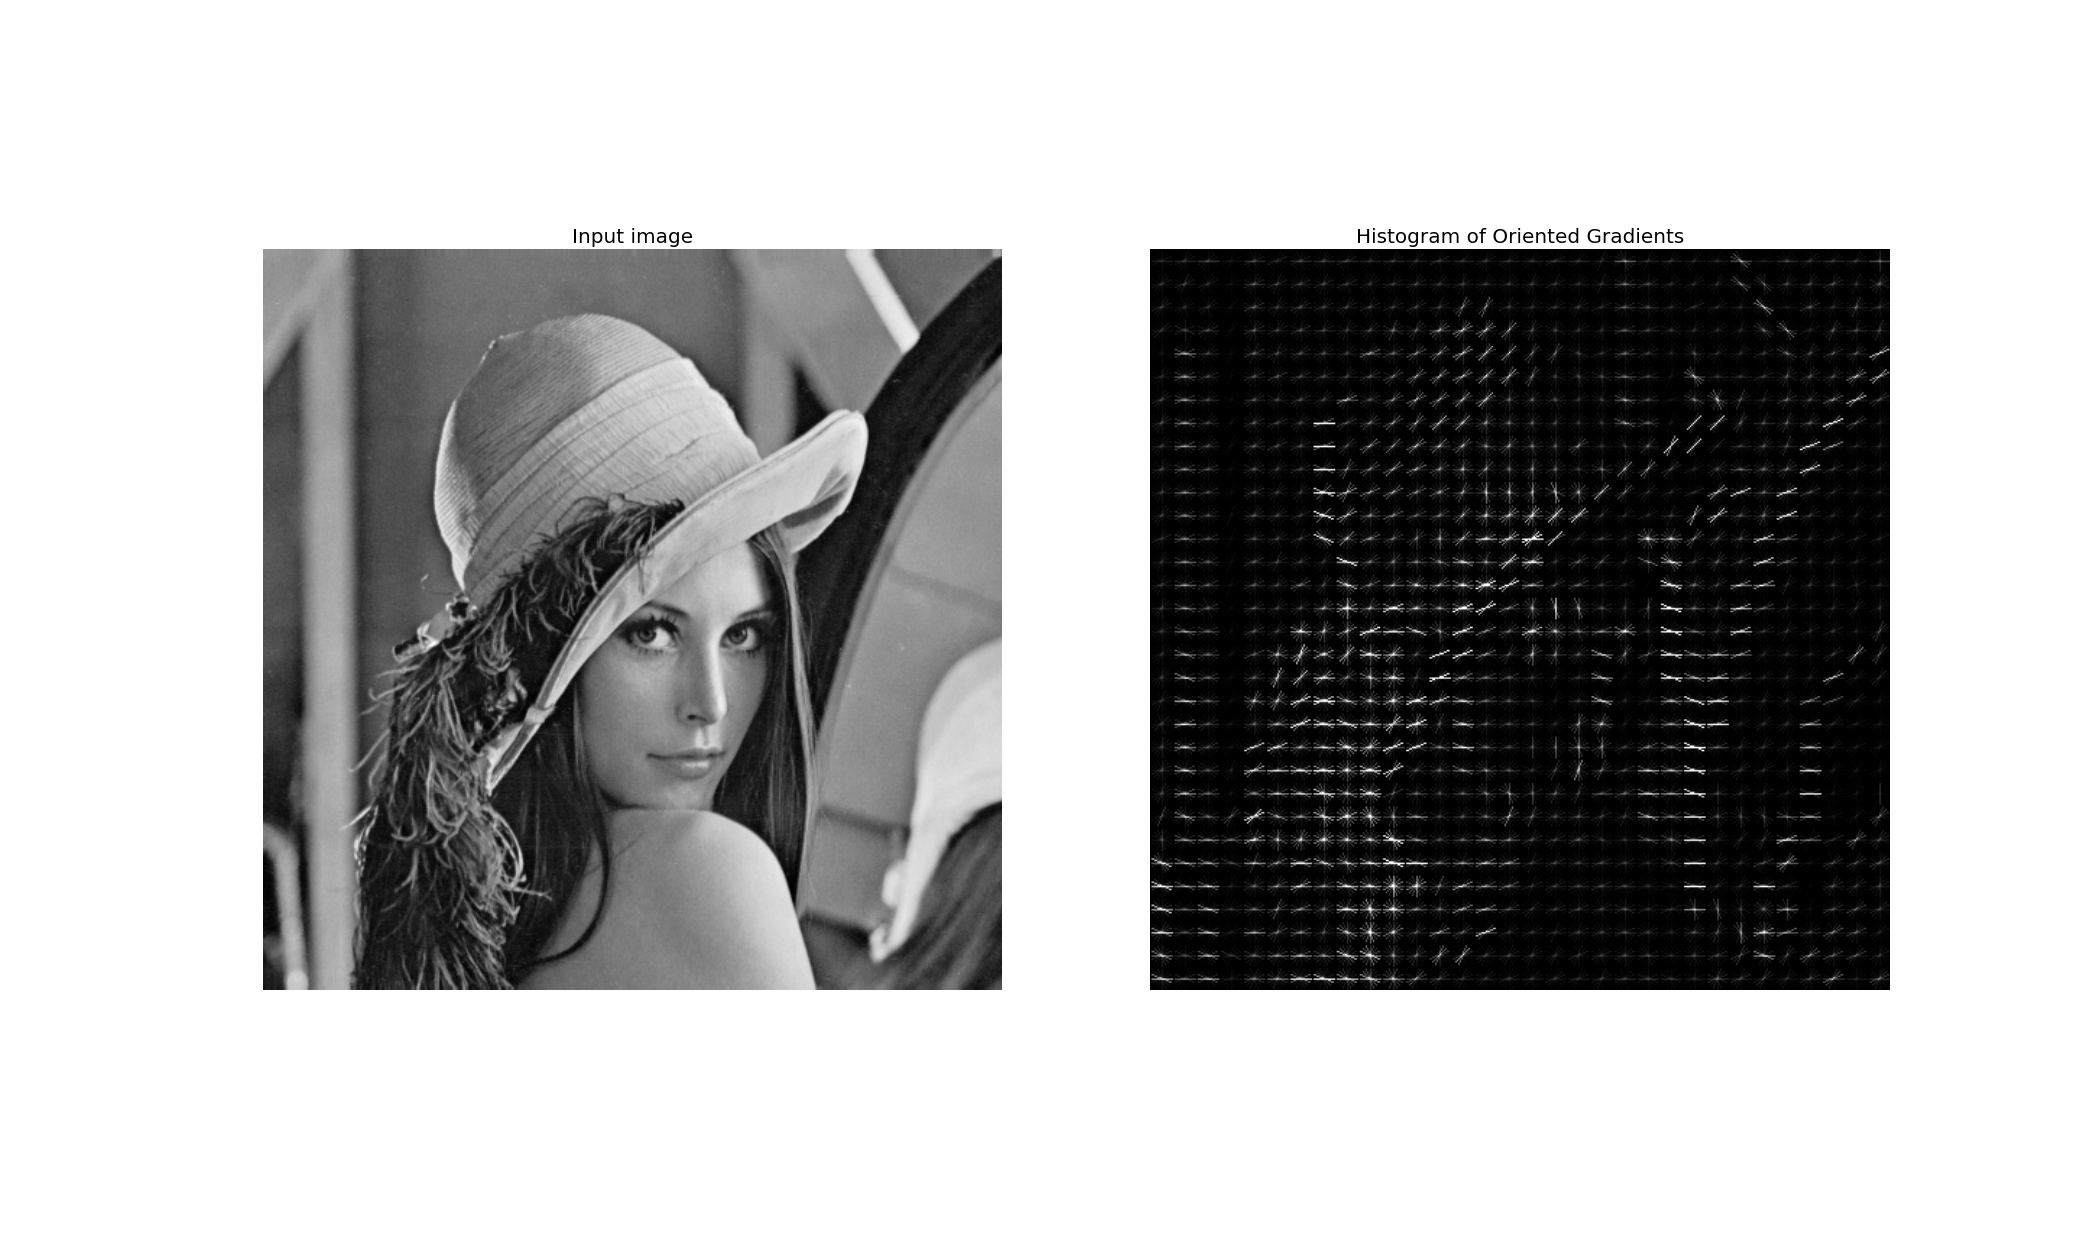
\includegraphics[width=\textwidth]{images/hog_lena_old.png}
    \caption{The image to the right shows the corresponding gradients of the cells from the input image (left). (TODO ska fixa en bild som illustrerar detta b\"{a}ttre)} 
    %TODO fixa bättre bild
    \label{fig:HOG_girl}
\end{figure}

There are several variations of HOG features and several of thus was already presented in the original paper\cite{HOG}.
In \cite{3Dhuman} the cells overlap each other which has the effect that things happening at the edge of a cell doesn't affect the features as much as in a non-overlapping grid where moving from one cell to another causes a greater change in the feature space.
In \cite{monocular} what is known as pyramid HOG is used where histograms from grids of different sizes are combined, the idea being that coarse grained cells contains information that is not accessible to fine grained cells and vice versa. 

\subsection{Smoothness, generativity and discriminativity}
\label{sec:featureproperties}
When evaluating image features we are interested to have the properties smoothness, generativity and discriminativity.
The first, smoothness, simply says that we would like for a small change in feature values to correspond to a small change in hand pose parameters.
This is as Akshaya notices far from the case for most image features \cite{akshayaMaster}.
In his results he tests linear transitions between hand poses which correspond to linear transitions in hand pose parameters (i.e. joint angles).
Ideally, the features would then change close to linearly which would essentially mean that it would be easier to find the mapping from feature to pose space using regression methods.
The other two aspects that we are interested in is concerned with what sort of mapping we have from pose space to feature space.
We would like to have a one-to-one mapping, but that is generally not possible and so we must relax that requirement and say that we want something as close as possible to a one-to-one mapping \cite{akshayaMaster}.
Generativity in this case means that we would like the same hand pose to generate the same image features, or at least to generate image features within a small subspace in the feature space.
We are also interested in discriminativity which is concerned with the other direction of the mapping.
That is, how unimodal the inverse mapping is.

%todo
%Figure på baksida och framsida av hand

\section{Discriminative vs Generative}
\label{sec:discgen}
Two quite different approaches to hand pose estimation is generative and discriminative models.
In discriminative models the mapping is estimated directly from training data.
This normally means that after the training is done, the estimation is quite fast since all that is required is to input the extracted feature values into the mapping and directly obtain the estimated pose.
It has, however, also been noted that discriminative approaches generally has lower accuracy, although they can to some degree compensate for that by being computationally more efficient\cite{monocular,recovering3D}.
The way the mapping from feature values to pose space is found is by fitting some regression method to the training data.
One might for instance use linear SVMs as in \cite{3Dhuman}, but might also go beyond that and use more advanced methods such as non-linear SVMs \cite{RGB}, RVMs \cite{regressionBased} or any other regression method.
An even easier approach is to use nearest neighbor (NN) algorithms to simply determine which data points are close in feature space and assume that they are also close in pose space.
In most situations the database is very large, for instance 90 000 in \cite{monocular}, meaning that exact NN is very expensive and an approximation is therefore used.
The approximative version (k-NN) normally returns $k$ data points that lies within a factor of the closest point.
Thus can then be interpolated in the pose space to get the estimated pose as in \cite{monocular}.
In \cite{recovering3D} different regression methods are tested with shape context features and the results shows that the regression method doesn't have that much of an impact although linear SVM performs slightly worse than RVM.
However, one quite ingenious method that is somewhat similar to the k-NN approximation which normally uses locality sensitive hashing (LSH) is to use parameter sensitive hashing (PSH) as in \cite{PSH} which allows one to find data points that likely is close in parameter space (i.e. pose space) which is precisely the goal of HPE.
The method builds on the idea to use hash functions which essentially have the property that close points in the pose space will correlate more than points that are not close in parameter space.
Even if the correlation is quite weak, multiple hash functions can be combined to form a good guess of which points are close in pose space.

Generative approaches uses a model of the hand that can be used to generate feature values from a pose.
The idea being that when a feature value is observed the problem is to find a pose that gives feature values as close as possible to the observed features.
However, because of the dimensionality of the problem MCMC (Markov Chain Monte Carlo) methods are used.
For instance, in \cite{fullDOF} a generative approach is used.
The study concerns hands interacting with objects and so the model contains both a model for the hand and a model for objects.
The estimation is done by minimizing a function using particle swarm optimization (PSO).
The function optimized was in this case formed by including two terms.
One term for the distance between the real features observed and the guessed poses feature, and one to penalize guesses where the object and hand intersect and therefore occupies the same physical space.
A generative approach is also used in \cite{cyberglove} although the approach is quite different seen as a cyberglove is used to get input and to determine different grasping types.
However, such approaches have the problem that the users motion becomes unnatural and limited.
Furthermore, it normally requires calibration and will generally be less accessible to the user.
%In \cite{pictorial} a discriminative approach is used for limb detection, but a generative method is used for pose estimation.  


\section{Multiple views and temporal constraints}
\label{sec:temporal}
One of the problems of hand pose estimation is ambiguity in the mapping from feature space to pose space.
Essentially, the mapping will be many-to-many even with a good image feature \cite{monocular}.
This depends on what image features are extracted, but the problem can also be attacked from another angle, namely by either adding additional views (i.e. cameras) or by adding temporal constraints in the estimation.
The idea behind using multiple views is to remove some of the ambiguity caused by self occlusion that is often dependent on viewing angle.
In \cite{exampleBased}, \cite{pictorial}, and \cite{regressionBased} both multiple and monocular views are tested and it is generally found that multiple views improves accuracy which is not surprising.
Campos notes that there are also different ways of using different views\cite{regressionBased}.
For instance, in \cite{regressionBased} a guess is made for each individual view whilst in \cite{exampleBased} the image features are combined before the estimation.  
However, if two views are too close to each other, it is not necessarily an improvement since the ability to distinguish depth would be limited and we can therefore still see that single view approaches can have important applications.
As noted in \cite{monocular} applications in robots makes monocular approaches important since robots are limited in the sense that they can't have cameras too far apart.

The idea with temporal constraints is that if we have a video of a gesture we would expect that the pose changes smoothly from frame to frame provided that the frames are close enough in time.
This can be difficult to achieve since the hand can move in about 5 $m/s$ and rotate in 300 $degrees/s$\cite{review}.
However, it is likely that the hand will only move at its fastest periodically and so even relatively slow frame rates can be useful.
The idea in temporal constraints is generally to weight different poses depending on how similar they are to the previous frames estimations.
However, because of ambiguity studies have been performed which uses several hypothesis for previous frames to avoid getting stuck at a wrong estimation \cite{review,nonparametric}.
A simpler approach used in \cite{monocular} weights data points obtained form a k-NN according to how similar they are to the previous estimation.
It is a bit more complex to introduce temporal constraints when using SVM or other none-example based methods.
In \cite{recovering3D} SVMs and RVMs are used and apart from managing to introduce the temporal constraint into the regression methods, they use two of the previous frames which allows for speed to be taken into account.
In some applications such as gesture recognition speed is even a necessity to capture the relevant information required to classify a certain gesture as in \cite{temporal}.
Even with time constraints it is normally required that we get an initial estimation, but we should also be able to reinitialize the pose estimation since a wrongly estimated frame can otherwise lead to wrongly estimated subsequent frames \cite{review}.

A recent study from 2013 presents a way to use depth sensors to improve hand estimations\cite{RGB}.
The method they use is mainly to compute one set of HOG features for the regular image and one set of HOG features for the depth-map of the image.
Additionally a fingertip detector is used to get fingertip position guesses.
Thus are then combined in a SVM and the results shows that using depth sensors does improve performance.




\begin{comment}

\subsection{A new descriptors}
%Slutgiltig schematisk bild över tanken
This thesis is about a novel way of getting hand descriptors.
However, before the descriptor is explained in more detail, the research from which this idea stems from must be explained.




\section{Classemes}
In a quite recent paper (2010) a new approach for object category regocnition was proposed\cite{classeme1}.
That is, given an image the classifier should classify the image as either belonging to or not belonging to a specific category.
The problem with many earlier approaches is that the classifiers doesn't scale well, and that learning new categories is very expensive or in fact impossible without relearning the whole classifier\cite{classeme1}.

The idea is to use a predetermined set of classifiers that one can combine to learn new categories.
The predetermined classifiers are learned by doing an web image search for a specific term to collect positive examples for that term, however, no human cleanup is used and so certain images might be rather unexpected.
If we now want to learn the new category duck we might be interested in what the classifiers for water and bird gives as output.
However, this is not entirely correct as the original classifiers are not supposed to have a semantic meaning, but rather use ancillary image characteristics.
For instance, a bird classifier might look for a V shaped object for the beak.
The authors points out that it is those ancillary image characteristics that is probably useful when combined and as can be seen in their results some of the new categories uses object classes that certainly doesn't seem to have any semantic connection\cite{classeme1}.

More specifically, when a new category is learned and when positive examples for that category is gathered one runs each of the original classifiers.
From those one obtains a binary vector where each element corresponds to the output of the corresponding classifier.
This vector is termed the descriptor vector and is all that is used when learning the new category.
It should be noted that to learn the original classifier a more advanced, namely $LP-\beta$, classifier is trained, but as noted in the paper those are trained prior to learning any novel categories and so it isn't of much importance if the orignal classifiers are computationally expensiv.

There have been subsequent papers on this idea, see \cite{classeme2,classeme3}.
They largerly use the same method, but with some modifications.
For instance, in \cite{classeme3} the classemes are learned as meta-classes meaning that they doesn't even have an apparant semantic meaning as in \cite{classeme1,classeme2}.

\subsection{A new descriptor}
This thesis introduces a novel descriptor that is loosely based on the idea of classemes from the previous section. 
However, the connection is somewhat vague as we first of all have a regression rather than classification problem.
The idea is however still to use multiple regressors instead of classifemes.
Assuming that a set of regressors has been choosen the goal would be that we could perform a regression to obtain a mapping from the descriptors to the pose space.
The quality of the reggresion function depends on how well suited the descriptor is in regard to smoothness, generativity and discriminativity as discussed in section~\ref{sec:featureproperties}.

So, how is these regressors formed.
This thesis will investigate if projections onto lines in the HOG space can serve as regressors.
However, it is far from obvious how these lines should be choosen.
Some of the questions one might ask are summarized below.
\begin{itemize}
\item
Should the lines be created from points close together in the HOG space and is there any requirement on the corresponding points in the pose space?
\item
Can we evaluate an individual line to tell if it is likely to be of use without using the whole descriptor?
\item
Should we only use two points for each line or can we use more than two? Might we in fact draw lines that doesn't go through any of the training points?
\item
It seems likely that a line that is far from a point doesn't help a lot in the prediction and so if possible it would likely be useful to weight which lines are used for the prediction.
\end{itemize}
These are some of the questions that will be investigated in this thesis and the experiments carried out are descriped in more detail in the section TODO %TODO metoddel
\end{comment}

\bibliography{references}{}
\bibliographystyle{plain}

\appendix
%\addappheadtotoc

\end{document}
